\documentclass[french,]{compterendu}
\usepackage{lmodern}
\usepackage{amssymb,amsmath}
\usepackage{ifxetex,ifluatex}
\usepackage{fixltx2e} % provides \textsubscript
\ifnum 0\ifxetex 1\fi\ifluatex 1\fi=0 % if pdftex
  \usepackage[T1]{fontenc}
  \usepackage[utf8]{inputenc}
\else % if luatex or xelatex
  \ifxetex
    \usepackage{mathspec}
  \else
    \usepackage{fontspec}
  \fi
  \defaultfontfeatures{Ligatures=TeX,Scale=MatchLowercase}
\fi
% use upquote if available, for straight quotes in verbatim environments
\IfFileExists{upquote.sty}{\usepackage{upquote}}{}
% use microtype if available
\IfFileExists{microtype.sty}{%
\usepackage{microtype}
\UseMicrotypeSet[protrusion]{basicmath} % disable protrusion for tt fonts
}{}
\usepackage[left=1.5cm,right=1.5cm,top=1.5cm,bottom=2cm]{geometry}
\usepackage{hyperref}
\hypersetup{unicode=true,
            pdftitle={Un titre évocateur et relativement court pour le compte-rendu},
            pdfauthor={Premier AUTEUR; Second AUTEUR},
            pdfborder={0 0 0},
            breaklinks=true}
\urlstyle{same}  % don't use monospace font for urls
\ifnum 0\ifxetex 1\fi\ifluatex 1\fi=0 % if pdftex
  \usepackage[shorthands=off,main=french]{babel}
\else
  \usepackage{polyglossia}
  \setmainlanguage[]{}
\fi
% Adding environment CSLReferences for compatibility with pandoc >= 2.8
% BEGIN
\newlength{\cslhangindent}
\setlength{\cslhangindent}{1.5em}
\newenvironment{CSLReferences}%
  {\setlength{\parindent}{0pt}%
  \everypar{\setlength{\hangindent}{\cslhangindent}}\ignorespaces}%
  {\par}
\newenvironment{cslreferences}%
  {\setlength{\parindent}{0pt}%
  \everypar{\setlength{\hangindent}{\cslhangindent}}\ignorespaces}%
  {\par}
% END
\usepackage{color}
\usepackage{fancyvrb}
\newcommand{\VerbBar}{|}
\newcommand{\VERB}{\Verb[commandchars=\\\{\}]}
\DefineVerbatimEnvironment{Highlighting}{Verbatim}{commandchars=\\\{\}}
% Add ',fontsize=\small' for more characters per line
\usepackage{framed}
\definecolor{shadecolor}{RGB}{248,248,248}
\newenvironment{Shaded}{\begin{snugshade}}{\end{snugshade}}
\newcommand{\AlertTok}[1]{\textcolor[rgb]{0.94,0.16,0.16}{#1}}
\newcommand{\AnnotationTok}[1]{\textcolor[rgb]{0.56,0.35,0.01}{\textbf{\textit{#1}}}}
\newcommand{\AttributeTok}[1]{\textcolor[rgb]{0.77,0.63,0.00}{#1}}
\newcommand{\BaseNTok}[1]{\textcolor[rgb]{0.00,0.00,0.81}{#1}}
\newcommand{\BuiltInTok}[1]{#1}
\newcommand{\CharTok}[1]{\textcolor[rgb]{0.31,0.60,0.02}{#1}}
\newcommand{\CommentTok}[1]{\textcolor[rgb]{0.56,0.35,0.01}{\textit{#1}}}
\newcommand{\CommentVarTok}[1]{\textcolor[rgb]{0.56,0.35,0.01}{\textbf{\textit{#1}}}}
\newcommand{\ConstantTok}[1]{\textcolor[rgb]{0.00,0.00,0.00}{#1}}
\newcommand{\ControlFlowTok}[1]{\textcolor[rgb]{0.13,0.29,0.53}{\textbf{#1}}}
\newcommand{\DataTypeTok}[1]{\textcolor[rgb]{0.13,0.29,0.53}{#1}}
\newcommand{\DecValTok}[1]{\textcolor[rgb]{0.00,0.00,0.81}{#1}}
\newcommand{\DocumentationTok}[1]{\textcolor[rgb]{0.56,0.35,0.01}{\textbf{\textit{#1}}}}
\newcommand{\ErrorTok}[1]{\textcolor[rgb]{0.64,0.00,0.00}{\textbf{#1}}}
\newcommand{\ExtensionTok}[1]{#1}
\newcommand{\FloatTok}[1]{\textcolor[rgb]{0.00,0.00,0.81}{#1}}
\newcommand{\FunctionTok}[1]{\textcolor[rgb]{0.00,0.00,0.00}{#1}}
\newcommand{\ImportTok}[1]{#1}
\newcommand{\InformationTok}[1]{\textcolor[rgb]{0.56,0.35,0.01}{\textbf{\textit{#1}}}}
\newcommand{\KeywordTok}[1]{\textcolor[rgb]{0.13,0.29,0.53}{\textbf{#1}}}
\newcommand{\NormalTok}[1]{#1}
\newcommand{\OperatorTok}[1]{\textcolor[rgb]{0.81,0.36,0.00}{\textbf{#1}}}
\newcommand{\OtherTok}[1]{\textcolor[rgb]{0.56,0.35,0.01}{#1}}
\newcommand{\PreprocessorTok}[1]{\textcolor[rgb]{0.56,0.35,0.01}{\textit{#1}}}
\newcommand{\RegionMarkerTok}[1]{#1}
\newcommand{\SpecialCharTok}[1]{\textcolor[rgb]{0.00,0.00,0.00}{#1}}
\newcommand{\SpecialStringTok}[1]{\textcolor[rgb]{0.31,0.60,0.02}{#1}}
\newcommand{\StringTok}[1]{\textcolor[rgb]{0.31,0.60,0.02}{#1}}
\newcommand{\VariableTok}[1]{\textcolor[rgb]{0.00,0.00,0.00}{#1}}
\newcommand{\VerbatimStringTok}[1]{\textcolor[rgb]{0.31,0.60,0.02}{#1}}
\newcommand{\WarningTok}[1]{\textcolor[rgb]{0.56,0.35,0.01}{\textbf{\textit{#1}}}}
\usepackage{longtable,booktabs}
\IfFileExists{parskip.sty}{%
\usepackage{parskip}
}{% else
\setlength{\parindent}{0pt}
\setlength{\parskip}{6pt plus 2pt minus 1pt}
}
\setlength{\emergencystretch}{3em}  % prevent overfull lines
\providecommand{\tightlist}{%
  \setlength{\itemsep}{0pt}\setlength{\parskip}{0pt}}
\setcounter{secnumdepth}{5}
% Redefines (sub)paragraphs to behave more like sections
\ifx\paragraph\undefined\else
\let\oldparagraph\paragraph
\renewcommand{\paragraph}[1]{\oldparagraph{#1}\mbox{}}
\fi
\ifx\subparagraph\undefined\else
\let\oldsubparagraph\subparagraph
\renewcommand{\subparagraph}[1]{\oldsubparagraph{#1}\mbox{}}
\fi

%%% Use protect on footnotes to avoid problems with footnotes in titles
\let\rmarkdownfootnote\footnote%
\def\footnote{\protect\rmarkdownfootnote}



%Mise en page
\usepackage[left=1.5cm,right=1.5cm,top=1.5cm,bottom=2cm]{geometry}
\usepackage{lastpage} %Pour numérotaion des pages
\usepackage{eso-pic} %pour l'image de fond de la page de garde
\usepackage{enumitem} %Pour personnaliser les listes à puces
\usepackage{fancyhdr}
\usepackage{xcolor}

%Gestion des tableaux
\usepackage{multirow}

%Divers
\usepackage{ifthen} %Gestion des instructions conditionnelles


\widowpenalty=10000
\clubpenalty=10000


%%%%%%%%%%%%%%%%%%%%%%%%%%%%%%%%%%%%%%%%%%%%%%%
%% Configuration des messages de type badbox %%
%%%%%%%%%%%%%%%%%%%%%%%%%%%%%%%%%%%%%%%%%%%%%%%

\widowpenalty=10000
\clubpenalty=10000


%%%%%%%%%%%%%%%%%%%%%%%%%%%%%%%
%% Definition environemments %%
%%%%%%%%%%%%%%%%%%%%%%%%%%%%%%%

%%%%%%%%%%%%%%%%%%%%%%%%%%%%%%%%%%%%%%%%%%%%
%% Désignation des variables de la classe %%
%%%%%%%%%%%%%%%%%%%%%%%%%%%%%%%%%%%%%%%%%%%%

  \title{Un titre évocateur et relativement court pour le compte-rendu}
    \author{Premier AUTEUR \\ Second AUTEUR}
      \date{04 janvier 2022}

\usepackage{booktabs}
\usepackage{longtable}
\usepackage{array}
\usepackage{multirow}
\usepackage{wrapfig}
\usepackage{float}
\usepackage{colortbl}
\usepackage{pdflscape}
\usepackage{tabu}
\usepackage{threeparttable}
\usepackage{threeparttablex}
\usepackage[normalem]{ulem}
\usepackage{makecell}
\usepackage{xcolor}

  \email{\href{mailto:premier.auteur@univ-reims.fr}{\nolinkurl{premier.auteur@univ-reims.fr}} \\ \href{mailto:second.auteur@univ-reims.fr}{\nolinkurl{second.auteur@univ-reims.fr}}}
%\email{\href{mailto:premier.auteur@univ-reims.fr}{\nolinkurl{premier.auteur@univ-reims.fr}}\href{mailto:second.auteur@univ-reims.fr}{\nolinkurl{second.auteur@univ-reims.fr}}}
\logouniv{logo_URCA.pdf}
\logoufr{logoUFR.pdf}
\date{04 janvier 2022}
\diplome{Licence Mathématiques Appliquées, 3\up{ème} année}
\anac{2019-2020}
\module{MA0606}
\enseig{Philippe Regnault}
\evaluation{Compte-rendu d'analyse}


%%%%%%%%%%%%%%%%%%%
%% Mise en forme %%
%%%%%%%%%%%%%%%%%%%


%Formatage en-têtes et pieds de pages
\pagestyle{fancy}
\fancyhead[L]{\small \thetitle}
\fancyhead[R]{}
\fancyfoot[l]{\small \theauthor}
\fancyfoot[C]{\small \it \theeval \ \themodule \ -- \theanac}
\fancyfoot[R]{\small \thepage\ / \pageref{LastPage}}
\renewcommand{\headrulewidth}{0.4pt}
\renewcommand{\footrulewidth}{0.4pt}

\fancypagestyle{plain}{%
\fancyhf{} % clear all header and footer fields
\fancyfoot[C]{\small \thepage\ / \pageref{LastPage}} % except the center
\renewcommand{\headrulewidth}{0pt}
\renewcommand{\footrulewidth}{0pt}}

\AtEndDocument{\thispagestyle{plain}}
% Pandoc header
\usepackage{booktabs}
\usepackage{longtable}
\usepackage{array}
\usepackage{multirow}
\usepackage{wrapfig}
\usepackage{float}
\usepackage{colortbl}
\usepackage{pdflscape}
\usepackage{tabu}
\usepackage{threeparttable}
\usepackage{threeparttablex}
\usepackage[normalem]{ulem}
\usepackage{makecell}
\usepackage{xcolor}


\usepackage{amsthm}
\newtheorem{theorem}{Theorem}[section]
\newtheorem{lemma}{Lemma}[section]
\newtheorem{corollary}{Corollary}[section]
\newtheorem{proposition}{Proposition}[section]
\newtheorem{conjecture}{Conjecture}[section]
\theoremstyle{definition}
\newtheorem{definition}{Definition}[section]
\theoremstyle{definition}
\newtheorem{example}{Example}[section]
\theoremstyle{definition}
\newtheorem{exercise}{Exercise}[section]
\theoremstyle{definition}
\newtheorem{hypothesis}{Hypothesis}[section]
\theoremstyle{remark}
\newtheorem*{remark}{Remark}
\newtheorem*{solution}{Solution}
\begin{document}

\AddToShipoutPictureBG*{
\includegraphics[width=\paperwidth,height=\paperheight]{FondURCA.png}}



\maketitle

\pagebreak

\begin{abstract}
Un paragraphe présentant de façon synthétique le contenu du compte-rendu.
\end{abstract}



{
\hypersetup{linkcolor=black}
\setcounter{tocdepth}{2}
\tableofcontents
}



\hypertarget{premiuxe8re-partie}{%
\section{Première partie}\label{premiuxe8re-partie}}

\begin{verbatim}
## Warning: le package 'knitr' a été compilé avec la version R 4.1.2
\end{verbatim}

\hypertarget{avec-une-premiuxe8re-sous-partie}{%
\subsection{Avec une première sous-partie}\label{avec-une-premiuxe8re-sous-partie}}

Le corps du document est rédigé selon la syntaxe de \emph{Markdown}. On peut mettre des expressions en \emph{italique} ou en \textbf{gras}, des blocs de code en ligne (non évalués) comme celui-ci \texttt{sample(1:49,\ 6)}, insérer des commentaires de base de page\footnote{Ceci est un commentaire de bas de page.}, des liens hypertexte comme \href{http://univ-reims.fr}{celui-là}, des expressions mathématiques du genre exprimées selon la syntaxe de \LaTeX du genre \(\cos(\theta) ^2 + \sin(\theta)^2 = 1\), voire les centrer comme ceci :
\[(a+b)^n = \sum_{k=0}^n {n \choose k} a^k b^{n-k}, \quad a,b \in \mathbb{C}, \quad n \in \mathbb{N}.\]

\hypertarget{puis-une-seconde}{%
\subsection{Puis une seconde}\label{puis-une-seconde}}

On peut également insérer des blocs de code R dont le rendu est paramétrable. Par exemple, le bloc suivant est affiché sans être évalué

\begin{Shaded}
\begin{Highlighting}[]
\FunctionTok{sample}\NormalTok{(}\DecValTok{1}\SpecialCharTok{:}\DecValTok{49}\NormalTok{, }\DecValTok{6}\NormalTok{)}
\end{Highlighting}
\end{Shaded}

tandis que la sortie suivante est affichée sans que le code exécuté n'apparaisse :

\begin{verbatim}
    Pearson's Chi-squared test

data:  un_tableau
X-squared = 2.8687, df = 6, p-value = 0.8251
\end{verbatim}

On peut également insérer du code R en ligne, qui sera remplacé par le résultat de son évaluation dans le document généré, par exemple, le résultat de \(3 \times 4\) vaut 12.

\hypertarget{deuxiuxe8me-partie}{%
\section{Deuxième partie}\label{deuxiuxe8me-partie}}

Le template \texttt{cr-urca} utilise le package \texttt{bookdown} apportant quelques fonctionnalités supplémentaires, dont la gestion des références croisées et des citations. La Figure \ref{fig:dotplotex} donne un exemple de graphique accompagné de sa légende.





\begin{figure}[ht!]

{\centering 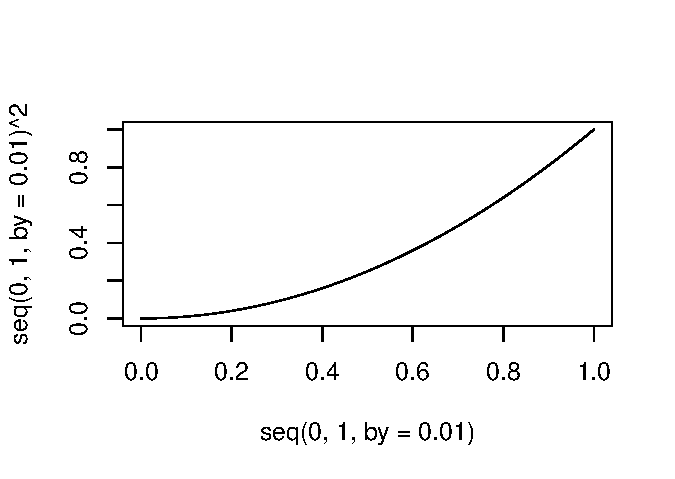
\includegraphics{Untitled_files/figure-latex/dotplotex-1} 

}

\caption{Un exemple de graphique produit par R, inséré et légendé grâce à \emph{R Markdown}. S'il y a lieu, on précise la source des donnés, la cohorte et on explique comment lire le graphique.
\textbf{Cohorte :} on peut insérer du code R dans la légende : il y a 101 points utilisé pour tracer ce graphique.
\textbf{Lecture :} Débrouillez-vous.}\label{fig:dotplotex}
\end{figure}

On peut faire de même pour les tableaux, comme illustré par la Table \ref{tab:tableex} pour laquelle on a utilisé le package \texttt{kableExtra} pour modifier le style du tableau.



\begin{verbatim}
Warning: le package 'kableExtra' a été compilé avec la
version R 4.1.2
\end{verbatim}

\begin{table}

\caption{\label{tab:tableex}Un exemple de tableau accompagné de sa légende.}
\centering
\begin{tabular}[t]{lrrrr}
\toprule
\textbf{ } & \textbf{1} & \textbf{2} & \textbf{3} & \textbf{4}\\
\midrule
\cellcolor{gray!6}{A} & \cellcolor{gray!6}{7} & \cellcolor{gray!6}{10} & \cellcolor{gray!6}{5} & \cellcolor{gray!6}{13}\\
B & 10 & 9 & 8 & 7\\
\cellcolor{gray!6}{C} & \cellcolor{gray!6}{12} & \cellcolor{gray!6}{8} & \cellcolor{gray!6}{3} & \cellcolor{gray!6}{8}\\
\bottomrule
\end{tabular}
\end{table}

Les équations mathématiques centrées et numérotées peuvent également être référencées, comme l'équation \eqref{eq:equationex}.

\begin{equation}
 \mathbb{H}(p_1, \dots, p_n) = \sum_{i=1}^n p_i \log p_i, \quad p_i \geq 0, i = 1, \dots, n \textrm{ and }  \sum_{i=1}^n p_i =1.
 \label{eq:equationex}
\end{equation}

De même, on peut faire référence aux théorèmes, propositions ou définitions que l'on déclare préalablement. Par exemple, le Théorème \ref{thm:theoex}.

\begin{theorem}{}
ffalse\{-91-80-121-116-104-97-103-111-114-101-97-110-32-116-104-101-111-114-101-109-93-\}\fi{}
\protect\hypertarget{thm:theoex}{}{\label{thm:theoex} \textbackslash iffalse (Pythagorean theorem) \fi{} }For a right triangle, if \(c\) denotes the length of the hypotenuse
and \(a\) and \(b\) denote the lengths of the other two sides, we have

\[a^2 + b^2 = c^2.\]
\end{theorem}

Pour citer un article, un ouvrage, une page web, etc, on remplit préalablement le fichier \texttt{biblio\_cr-urca.bib} en déclarant les références dans la syntaxe de \emph{Bibtex} puis on insère la citation. Pour plus d'information sur le fonctionnement de \emph{R Markodown}, on pourra consulter (\protect\hyperlink{ref-rmarkdown_refbook2018}{Xie, Allaire, and Grolemund 2018}).

\hypertarget{appendix-annexes}{%
\appendix}


\hypertarget{annexes}{%
\section{Annexes}\label{annexes}}

On peut également ajouter une ou des partie(s) annexe(s) au document, permettant par exemple de détailler les procédures statistiques employées.

\hypertarget{bibliographie}{%
\section*{Bibliographie}\label{bibliographie}}
\addcontentsline{toc}{section}{Bibliographie}

\hypertarget{refs}{}
\begin{CSLReferences}{1}{0}
\leavevmode\vadjust pre{\hypertarget{ref-rmarkdown_refbook2018}{}}%
Xie, Yihui, J. J. Allaire, and Garrett Grolemund. 2018. \emph{R Markdown: The Definitive Guide}. Boca Raton, Florida: Chapman; Hall/CRC. \url{https://bookdown.org/yihui/rmarkdown}.

\end{CSLReferences}

% % 
% % 
% % 
% 
% 
% 
% 

\end{document}
